\documentclass[tikz]{standalone}

\usepackage{amssymb,amsmath}
\usepackage{fourier}
\usepackage{inconsolata}

\usetikzlibrary{fit,positioning,backgrounds}

\makeatletter
\pgfdeclaregenericanchor{top base}{%
    \csname pgf@anchor@#1@north\endcsname
    \pgf@anchor@generic@top@base@main
}
\pgfdeclaregenericanchor{top base west}{%
    \csname pgf@anchor@#1@north west\endcsname
    \pgf@anchor@generic@top@base@main
}
\pgfdeclaregenericanchor{top base east}{%
    \csname pgf@anchor@#1@north east\endcsname
    \pgf@anchor@generic@top@base@main
}
\def\pgf@anchor@generic@top@base@main{%
    {%
        \pgfmathsetlength\pgf@ya{\pgfkeysvalueof{/pgf/outer ysep}}%
        \advance\pgf@y-\pgf@ya
        \pgfmathsetlength\pgf@ya{\pgfkeysvalueof{/pgf/inner ysep}}%
        \advance\pgf@y-\pgf@ya
        \pgf@ya=0pt
        \pgfutil@loop
        \ifdim\pgf@y>\baselineskip
        \advance\pgf@y-\baselineskip
        \advance\pgf@ya\baselineskip
        \pgfutil@repeat
        \global\pgf@y=\pgf@ya
    }%
}
\makeatother

\begin{document}
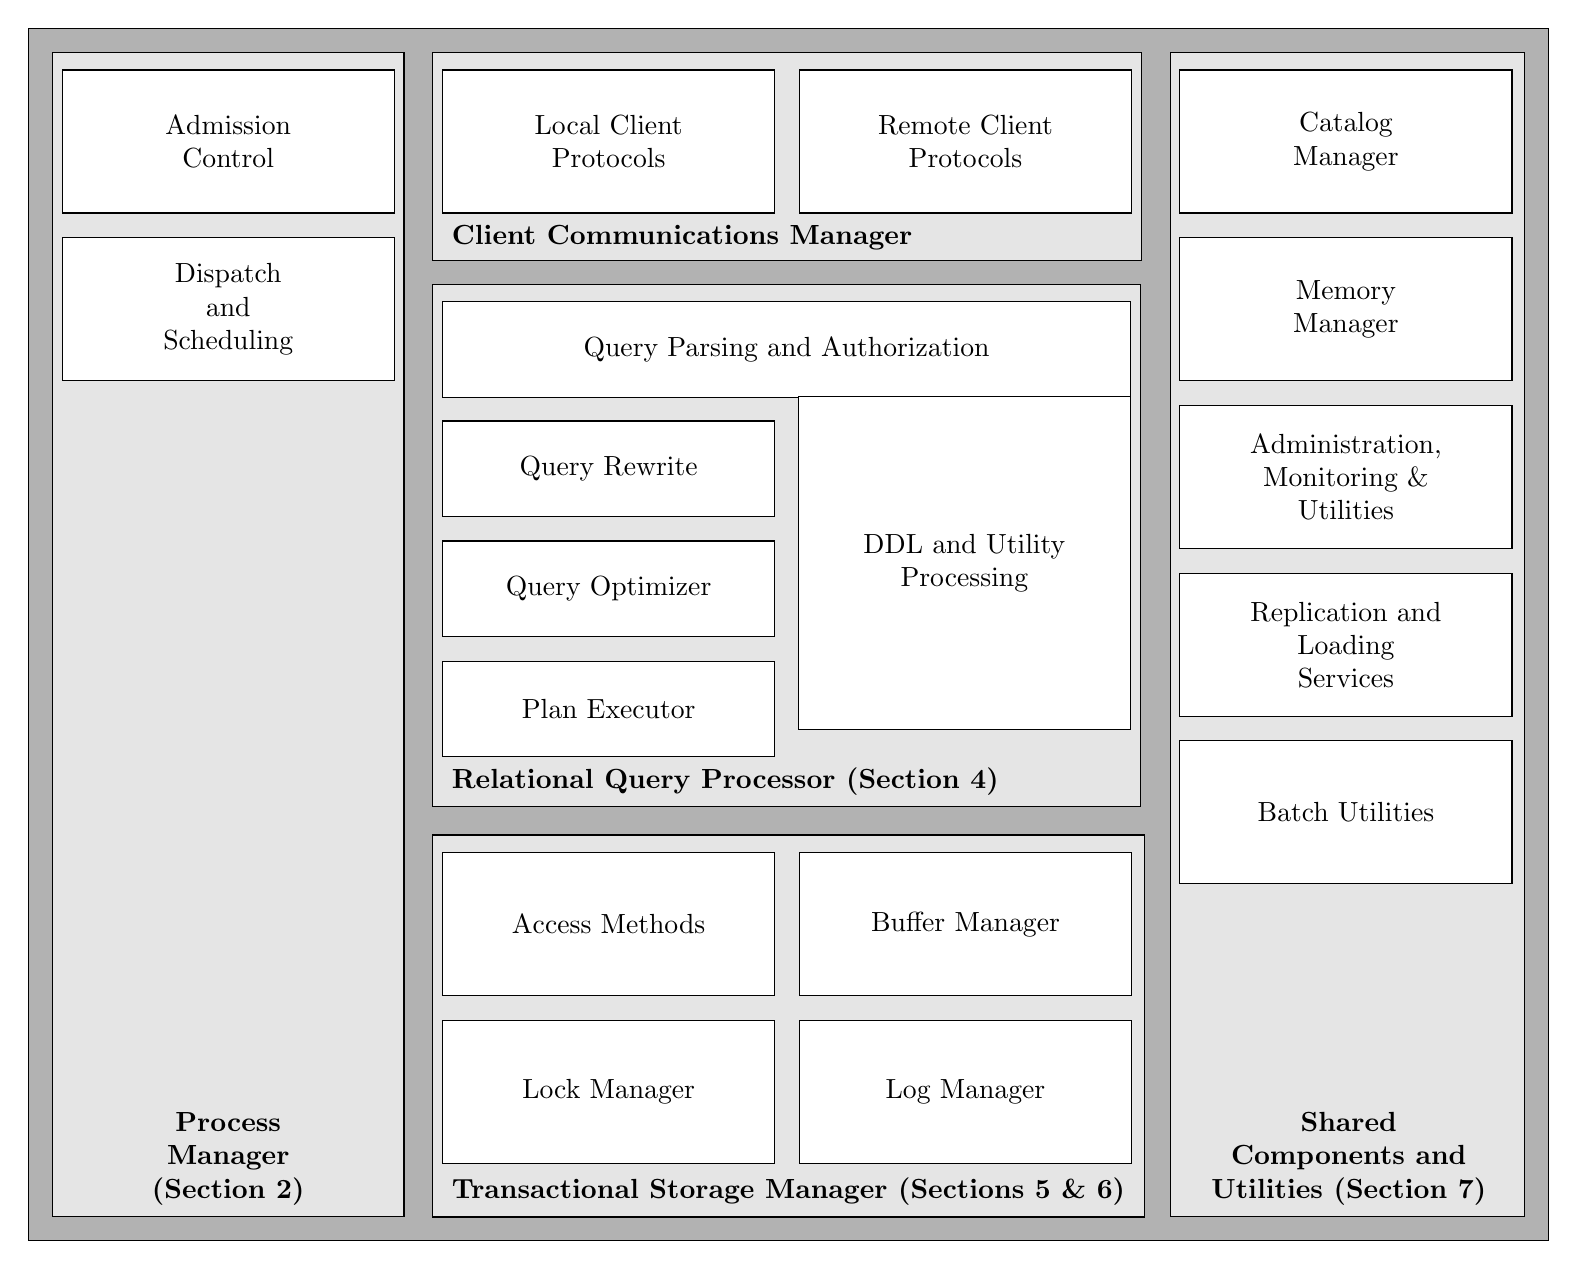
\begin{tikzpicture}[
  node distance=3mm,
  title/.style={font=\bfseries},
  box/.style={draw,minimum width=12em,minimum height=12ex,align=center,fill=white},
  box2/.style={draw,minimum width=12em,minimum height=8ex,align=center,inner ysep=0em,fill=white},
]

%%%%%%%%%%%%%%%
%%%%%%%%%%%%%%%
\node (l1) [box] {Admission\\Control};
\node [box,below=of l1] {Dispatch\\and\\Scheduling};

%%%%%%%%%%%%%%%
%%%%%%%%%%%%%%%
\node (cl1) [box,right={6mm of l1}] {Local Client\\Protocols};
\node (cr1) [box,right=of cl1] {Remote Client\\Protocols};
\node (ct1) [title,anchor=top base west,at=(cl1.top base west),yshift=-12ex] {Client Communications Manager};
\node [draw,fit=(cl1)(cr1)(ct1),yshift=1mm] {};

%%%%%%%%%%%%%%%
\node (c2) [box2,minimum width=24em+3mm,anchor=top base west,at=(ct1.top base west),yshift=-2ex-3mm-4mm] {Query Parsing and Authorization};
\node (cl2) [box2,anchor=top base west,at=(c2.top base west),yshift=-8ex-3mm] {Query Rewrite};
\node (cl3) [box2,below=of cl2] {Query Optimizer};
\node (cl4) [box2,below=of cl3] {Plan Executor};
\node (cr2) [box2,minimum height=24ex+6mm,anchor=top base west,at=(cl2.top base west),xshift=12em+3mm,yshift=2.8mm] {DDL and Utility\\Processing};
\node (ct2) [title,anchor=top base west,at=(cl4.top base west),yshift=-8ex-1mm] {Relational Query Processor (Section 4)};
\node [draw,fit=(c2)(ct2),yshift=1mm] {};

%%%%%%%%%%%%%%%
\node (cl5) [box,anchor=top base west,at=(ct2.top base west),yshift=-2ex-3mm-4mm] {Access Methods};
\node (cr5) [box,right=of cl5] {Buffer Manager};
\node (cl6) [box,below=of cl5] {Lock Manager};
\node (cr6) [box,right=of cl6] {Log Manager};
\node (ct3) [title,anchor=top base west,at=(cl6.top base west),yshift=-12ex-3mm] {Transactional Storage Manager (Sections 5 \& 6)};
\node [draw,fit=(cl5)(cr5)(ct3),yshift=1mm] {};

%%%%%%%%%%%%%%%
%%%%%%%%%%%%%%%
\node (r1) [box,right=of cr1,xshift=3mm] {Catalog\\Manager};
\node (r2) [box,below=of r1] {Memory\\Manager};
\node (r3) [box,below=of r2] {Administration,\\Monitoring \&\\Utilities};
\node (r4) [box,below=of r3] {Replication and\\Loading\\Services};
\node (r5) [box,below=of r4] {Batch Utilities};

%%%%%%%%%%%%%%%
%%%%%%%%%%%%%%%

\node (lt) [minimum width=12em,title,align=center,anchor=top base east,left=6mm of ct3,yshift=\baselineskip] {Process\\Manager\\(Section 2)};
\node (l) [draw,fit=(l1)(lt),yshift=1mm] {};

\node (rt) [minimum width=12em,title,align=center,anchor=top base west,right=6mm of ct3,yshift=\baselineskip] {Shared\\Components and\\Utilities (Section 7)};
\node (r) [draw,fit=(r1)(rt),yshift=1mm] {};

\begin{scope}[on background layer]
\node [draw,inner sep=3mm,fill=black!30,fit=(l)(r)] {};
\end{scope}
\begin{scope}[on background layer]
\node [fill=black!10,draw,fit=(l1)(lt),yshift=1mm] {};
\node [fill=black!10,fit=(r1)(rt),yshift=1mm] {};
\node [fill=black!10,fit=(cl1)(cr1)(ct1),yshift=1mm] {};
\node [fill=black!10,fit=(c2)(ct2),yshift=1mm] {};
\node [fill=black!10,fit=(cl5)(cr5)(ct3),yshift=1mm] {};
\end{scope}

\end{tikzpicture}
\end{document}
